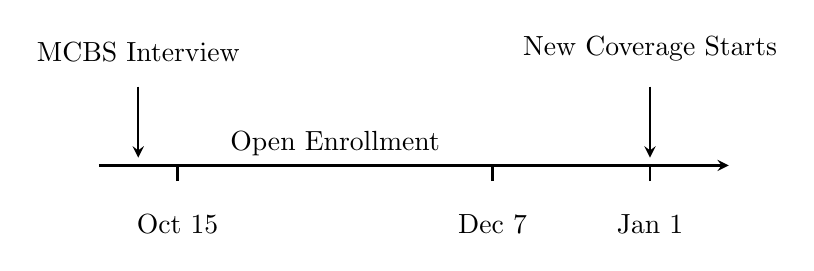
\begin{tikzpicture}
    % Draw horizontal line
    \draw[->, >=stealth, thick] (0,0) -- (8,0);
    
    % Draw vertical lines for the dates
    \draw[thick] (1,-0.2) -- (1,0);
    \draw[thick] (5,-0.2) -- (5,0);
    \draw[thick] (7,-0.2) -- (7,0);
    
    % Place the date labels
    \node[align=center, below] at (1,-0.5) {Oct 15};
    \node[align=center, below] at (5,-0.5) {Dec 7};
    \node[align=center, below] at (7,-0.5) {Jan 1};

    % Add "Open Enrollment" label above the line between Oct 15 and Dec 7
    \node[align=center, above] at (3,0) {Open Enrollment};

    % Add arrow and label for "MCBS Interview" to the left of Oct 15
    \draw[->, >=stealth, thick] (0.5,1) -- (0.5,0.1);
    \node[align=center, above] at (0.5,1.2) {MCBS Interview};

    % Add arrow and label for "New Coverage Starts" at Jan 1
    \draw[->, >=stealth, thick] (7,1) -- (7,0.1);
    \node[align=center, above] at (7,1.2) {New Coverage Starts};
\end{tikzpicture}